%
% Niniejszy plik stanowi przykład formatowania pracy magisterskiej na
% Wydziale MIM UW.  Szkielet użytych poleceń można wykorzystywać do
% woli, np. formatujac wlasna prace.
%   
% Zawartosc merytoryczna stanowi oryginalnosiagniecie
% naukowosciowe Marcina Wolinskiego.  Wszelkie prawa zastrzeżone.
%
% Copyright (c) 2001 by Marcin Woliński <M.Wolinski@gust.org.pl>
% Poprawki spowodowane zmianami przepisów - Marcin Szczuka, 1.10.2004
% Poprawki spowodowane zmianami przepisow i ujednolicenie 
% - Seweryn Karłowicz, 05.05.2006
% Dodanie wielu autorów i tłumaczenia na angielski - Kuba Pochrybniak, 29.11.2016

% dodaj opcję [licencjacka] dla pracy licencjackiej
% dodaj opcję [en] dla wersji angielskiej (mogą być obie: [licencjacka,en])
\documentclass[licencjacka,en]{pracamgr}

\usepackage{graphicx} %package to manage images
\usepackage{url}
\graphicspath{ {./images/} }
\usepackage[utf8]{inputenc}
\usepackage[rightcaption]{sidecap}

\usepackage{wrapfig}

% Dane magistranta:
% \autor{Adam Deryło, Adrian Hess, Magdalena Pałkus, Michał Skwarek}{34234234}

% Dane magistrantów:
\autor{Adam Deryło}{432952}
\autori{Adrian Hess}{431481}
\autorii{Magdalena Pałkus}{421537}
\autoriii{Michał Skwarek}{418426}
%\autoriv{Autor nr Cztery}{432145}
%\autorv{Autor nr Pięć}{342011}

\title{GPU acceleration of CCSDS Rice decoding}
\titlepl{Akcerleracja GPU dekodowania CCSDS Rice}

%\tytulang{An implementation of a difference blabalizer based on the theory of $\sigma$ -- $\rho$ phetors}

%kierunek: 
% - matematyka, informacyka, ...
% - Mathematics, Computer Science, ...
\kierunek{Computer Science}

% informatyka - nie okreslamy zakresu (opcja zakomentowana)
% matematyka - zakres moze pozostac nieokreslony,
% a jesli ma byc okreslony dla pracy mgr,
% to przyjmuje jedna z wartosci:
% {metod matematycznych w finansach}
% {metod matematycznych w ubezpieczeniach}
% {matematyki stosowanej}
% {nauczania matematyki}
% Dla pracy licencjackiej mamy natomiast
% mozliwosc wpisania takiej wartosci zakresu:
% {Jednoczesnych Studiow Ekonomiczno--Matematycznych}

% \zakres{Tu wpisac, jesli trzeba, jedna z opcji podanych wyzej}

% Praca wykonana pod kierunkiem:
% (podać tytuł/stopień imię i nazwisko opiekuna
% Instytut
% ew. Wydział ew. Uczelnia (jeżeli nie MIM UW))
\opiekun{Paweł Gora\\
  Faculty of Mathematics, Informatics and Mechanics, University of Warsaw\\
  }

% miesiąc i~rok:
\date{Jan 2023}

%Podać dziedzinę wg klasyfikacji Socrates-Erasmus:
\dziedzina{ 
%11.0 Matematyka, Informatyka:\\ 
%11.1 Matematyka\\ 
% 11.2 Statystyka\\ 
11.3 Informatics, Computer Science \\ 
%11.3 Informatyka\\ 
%11.4 Sztuczna inteligencja\\ 
%11.5 Nauki aktuarialne\\
%11.9 Inne nauki matematyczne i informatyczne
}

%Klasyfikacja tematyczna wedlug AMS (matematyka) lub ACM (informatyka)
\klasyfikacja{D. Software\\
  D.1.3. Concurrent Programming\\
  I.4.2. Compression (Coding) \\ }

% Słowa kluczowe:
\keywords{CCSDS Rice coding, GPU, Compute Unified Device Architecture (CUDA)}

% Tu jest dobre miejsce na Twoje własne makra i~środowiska:
\newtheorem{defi}{Definicja}[section]

% koniec definicji

\begin{document}
\maketitle

%tu idzie streszczenie na strone poczatkowa
\begin{abstract}
	TBD
\end{abstract}

\tableofcontents
%\listoffigures
%\listoftables

\chapter{Introduction}
\section{Background and motivation}
Machine learning (ML) has rapidly become a crucial tool for solving complex problems in a variety of domains, including computer vision, natural language processing, and speech recognition. However, ML pipelines can often experience significant bottlenecks due to multi-stage data processing pipelines that include loading, decoding, cropping, resizing, and other augmentations. This is particularly true when these processing steps are executed on a CPU, which is frequently the case. Since most of the machine learning training is already GPU accelerated due to ML workloads having a highly parallel nature, it is a natural progression to solve data processing bottlenecks by harnessing GPU acceleration.

One such bottleneck is decompression of RICE coded data, which is one of the most commonly used compression algorithms used in astronomy and astrophysics. Currently, there are only CPU-based solutions for decoding RICE compressed data. This, substantially hinders application of machine learning solutions in astronomy, especially considering the massive amount of training data already stored in RICE compressed algorithm as well as being produced by observatories all around the world. To illustrate, just Solar Dynamics Observatory (SDO), with limited bandwidth due to being a satellite, is producing 130 megabits of rice coded data per second, that is 500 TB per year.

\section{Problem statement}
The problem at hand is that the current RICE decompression algorithm is a computationally intensive and cannot keep up with the demand for high throughput and real-time processing. The goal of this project is to design and develop a GPU-based RICE decompression algorithm that can significantly accelerate the decompression process and improve the speed, efficiency, and scalability of ML pipelines in astronomy applications.

\section{Research objectives}
The main objectives of this thesis are as follows:

\begin{itemize}
	\item To study the existing literature on GPU acceleration of data compression and RICE decompression.
	\item To analyze the performance of RICE decompression on a CPU and a GPU.
	\item To design and implement a GPU-accelerated RICE decompression algorithm.
	\item To evaluate the performance of the GPU-accelerated RICE decompression algorithm and compare it with the CPU-based RICE decompression algorithm.
	\item And finally, to incorporate findings into NVIDIA Data Loading Library (DALI), so machine learning as well as the astronomy community can utilize our findings.
\end{itemize}

\section{Thesis structure}
In this thesis, we present our attempts at parallelizing the RICE decompression algorithm and CUDA-based implementations of our findings.

Chapter 2 aims to define and explain key terms for our problem space, including the RICE algorithm itself. In the following chapter, we review previous work on the subject. We then present our solution architecture and how it ties into NVIDIA's open-source data loading framework called DALI. Additionally, we introduce the Compute Unified Device Architecture (CUDA) to the reader. In Chapter 5, we propose a parallel implementation of the algorithm on GPU with details. Chapter 6 presents our performance and speedup results. Finally, in Chapter 7, we summarize our findings and conclude the thesis.

\chapter{Key terms}\label{r:pojecia}


\section{RICE}
The RICE algorithm is a well-known, lossless, bit-wise data compression algorithm, that uses a set of variable-length codes to compress data. As a lossless data compression algorithm, RICE enable to retrieve full data from compressed form, without losing any part of original data. Bit-wise algorithm operates on operate on single bits (in difference on byte-wise, which operate on single bytes) enable a greater degree of compression, due to the smaller granularity of the data on which they work. The essence of this algorithm is using these codes to change symbols that are expected to be more frequent to shorter code words. The algorithm works on data blocks that are encoded independently, so it is not needed to transfer some information between different packets. It improves performance and makes RICE algorithm performance independent of data packet size. Image encoding by RICE algorithm is carried out by dividing the image into blocks of pixels, then applies a predictive coding technique for compute and encode differences between the predicted value and the actual value, using a variant of the Golomb coding. This variant using fixed-length prefix of binary zeros followed by a unary code to represent the quotient and the remainder of the difference value. While in Golomb coding, there is a variable parameter that means, how many bits are are needed to write the remainder of division by a fixed number, in the RICE algorithm, data block always have constant size, so number of needed bits is constant, and it is always a power of two. This fact causes, that there can be used simple arithmetic bite-shifting operation, that work in constant time, what accelerate compression process.
Prefix size typically depend on the characteristics of the image being compressed. \hfill \break

The RICE algorithm consists of two main parts: a preprocessor and an adaptive entropy coder:
\begin{itemize}
	\item The preprocessor is responsible for data processing, before proper compression. This part of algorithm converts input data into preprocessed samples, and passes them to Adaptive Entropy Coder
	\item Adaptive Entropy Coder assigns shorter codes to symbols that occur more frequently and longer codes to symbols that occur less frequently. This part of algorithm convert preprocessed samples into finally encoded bit sequence.
\end{itemize}

\hfill \break
\hfill \break
\hfill \break
\hfill \break
This process can be ilustrated into following figure:
\hfill \break
\hfill \break
\centerline{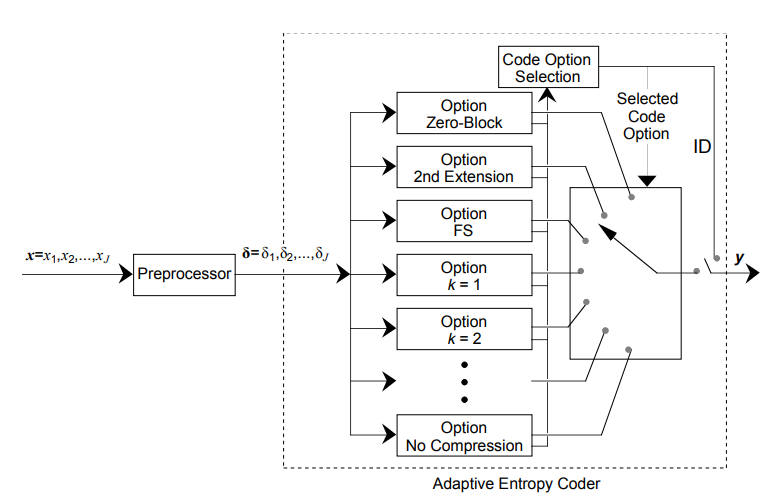
\includegraphics[scale=1.05]{RICE_encoder_architecture}}

\section{FITS}
The Flexible Image Transport System (FITS) format is an openly documented digital file format that is commonly
utilized in the field of astronomy for storing and transferring scientific data. The International Astronomical Union FITS Working Group (IAU-FWG) is responsible for developing and maintanancing FITS format, although worldwide astromers' community have major influence on its development direction. FITS format was designed for long-term usage, and enables support for this purpose, like backwards compatibility and standarization. FITS files
typically contain images, data cubes, tables of observational data, usually with its associated metadata. Storing metadata enable to store data such as observation date, instrument name and coordinates.
One of the key characteristics of FITS is its ability to store multiple data arrays in a single file, which
allows for the efficient storage and transfer of large data sets.
A FITS files are composed of the following FITS structures, in the order listed:
\begin{itemize}
	\item Primary header and data unit (HDU).
	\item Conforming Extensions (optional).
	\item Other special records (optional, restricted).
\end{itemize}
Thus, files usually resemble the following schema:
\hfill \break
\hfill \break

\centerline{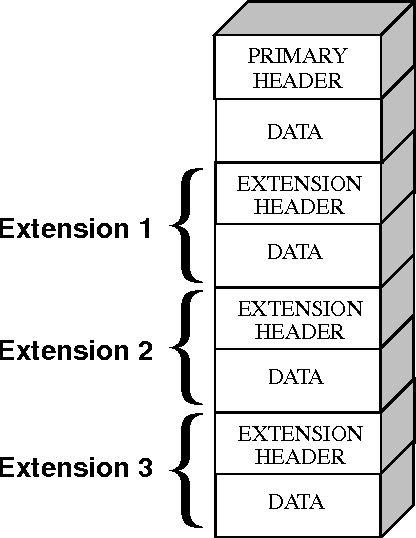
\includegraphics[scale=0.3]{fits}}

\hfill \break

Where, all headers, including the primary one, contain relevant metadata as a list of keys and value pairs.
Furthermore, according to the most recent FITS standard published by NASA, there are three types of standard extensions:
\begin{itemize}
	\item IMAGE extensions.
	\item TABLE ASCII-table extensions; and
	\item BINTABLE binary-table extensions
\end{itemize}

\section{Astronomical image compression}
TODO:\\
1.Why compress at all? \\
2.Tile compression convention.\\
3.Review of employed compression algorithms. (and why rice is the best) \\

Soruces:
https://heasarc.gsfc.nasa.gov/fitsio/fpack/O1.5.pdf  (1)
https://arxiv.org/pdf/0903.2140.pdf
(2,3)

\chapter{Related work}

\section{Overview of the problem space}
The acceleration of the Golomb-Rice algorithm has garnered significant attention in the literature, with most of the work focusing on the compression side of the problem. In particular, researchers have extensively studied Golomb parameter selection due to its critical role in determining achieved compression ratios. However, with respect to throughput acceleration, the majority of the research has focused on implementing FPGA-based hardware acceleration for both compression and decompression. Notably, some software (CPU-based) approaches have been implemented, leveraging input format to achieve decoding throughput improvements from 1 Gbps to 4 Gbps. (source needed)\\

Regarding GPU-based acceleration, Xianyun Wu et al. evaluated the feasibility of GPU acceleration for the coding side of the problem in their study "Is the CCSDS Rice Coding Suitable for GPU Massively Parallel Implementation?" The authors achieved a six-fold speedup over the single-threaded CPU counterpart and concluded that CCSDS Rice coding contains numerous flow control instructions, significantly affecting the instruction throughput. These findings highlight the potential benefits of GPU-based acceleration for the coding side of the problem, but also suggest that further work is necessary to optimize CCSDS Rice coding for efficient GPU-based implementations.

\newpage
\section{Current RICE decoding solutions in context of FITS}
To the best of our knowledge, the industry standard for compression and decompression of CCSDS Rice coded FITS files is achieved through standalone programs, fpack and funpack. These programs offer a unique advantage as they directly read and write the compressed FITS image format, eliminating the need for creating an uncompressed version of the file. Additionally, fpack and funpack rely on the aforementioned tile compression convention and support multiple compression algorithms, including Hcompress, GZIP, and IRAF, apart from RICE \cite{funpack}. Both programs are included with CFITSIO, a FITS File Subroutine Library that is maintained by NASA’s High-Energy Astrophysics Science Archive Research Center (HEASARC)\cite{cfitsio}.\\

Regarding machine learning and data science workflows, where python is a prevailing programming language, either astropy or fitsio packages are mainly utilized. While fitsio is simply a Python wrapper for CFITSIO \cite{fitsio}, astropy builds upon the PyFits package and is thus a standalone Python implementation of fitsio. Nevertheless, when it comes to compression, astropy accesses CFITSIO to support the FITS Tile Compression convention \cite{astropy}, what in the end makes them equivalent in terms of throughput in most cases. On that note, fitsio is shown to outperform astropy on the data sets consisting mainly of small files ($\sim $ 0.3MB) \cite{astropy vs fitsio}, thus it will be used for various Python based benchmarks. \\

In summary, the fitsio and astropy packages offer convenient interfaces for accessing FITS files and decompressing CCSDS Rice encoded data in Python-based workflows. However, it should be noted that all of these packages rely on the same CPU-based RICE decompression algorithm implemented by funpack. While this algorithm has proven to be effective in achieving high compression ratios for a wide range of data types, it is limited in terms of its processing speed and throughput. As such, there is a growing interest in exploring alternative solutions that leverage emerging hardware technologies such as GPUs and FPGAs to accelerate the RICE decompression process. Such solutions have the potential to significantly improve the performance and efficiency of CCSDS Rice encoding and decoding in various domains, including machine learning, data science, and space science.

\chapter{Context}\label{r:losers}

\section{NVIDIA}
TODO: Explain what NVIDIA does and their intrest in scientific computing. \\

NVIDIA Corporation is a technology company known for designing and manufacturing wgraphics processing units (GPUs). Its professional line of GPUs are used in workstations for applications in such fields as architecture, engineering and construction, media and entertainment, automotive, scientific research, and manufacturing design. \\

In addition to designing hardware, NVIDIA has made significant efforts to develop software tools and libraries that facilitate the use of their GPUs in scientific computing. Among these efforts, CUDA stands out as one of the most notable contributions. CUDA, which stands for Compute Unified Device Architecture, is a parallel computing platform and programming model that enables researchers to harness the power of GPUs for scientific computing tasks. With CUDA, developers can write programs in C, C++, and Fortran that can take advantage of the parallelism of GPUs to accelerate computations. This has led to significant performance improvements for many scientific computing applications, including those in the fields of astrophysics, computational biology, and machine learning. \\

To further support the use of GPUs in scientific computing, NVIDIA provides a range of software libraries that are optimized for use with CUDA. These include cuBLAS, cuFFT, and cuSPARSE, which provide high-performance implementations of common linear algebra, signal processing, and sparse matrix operations that are essential for many scientific computing applications. By offering these libraries, NVIDIA has made it easier for researchers and developers to take advantage of the power of GPUs in scientific computing. \\


%%\begin{itemize}
%\item {https://www.nvidia.com/en-us/about-nvidia/}
%\item {https://research.nvidia.com/publication/2021-12_evolution-graphics-processing-unit-gpu}
%\item https://www.nvidia.com/en-us/technologies/
%\item https://www.nvidia.com/en-us/data-center/ampere-architecture/
%\item https://developer.nvidia.com/cuda-zone
%\end{itemize}

\section{GPU Programming and CUDA}
Explain the field of GPU programing.

\section{DALI}
Expalain what is DALI and it's graph like architecture for data pre-processing aimed at helping with ML workflows. \\

DALI is a set of highly optimized building blocks and an execution engine to accelerate input data pre-processing for Deep Learning (DL) applications. DALI provides performance and flexibility for accelerating different data pipelines. DALI defines data pre-processing pipeline as a dataflow graph, with each node representing a data processing Operator. DALI has 3 types of Operators as follows: CPU: accepts and produces data on CPU; Mixed: accepts data from CPU and produces the output at the GPU side; GPU: accepts and produces data on the GPU.\\

The flexibility of DALI also allows it to seamlessly integrate with popular deep learning frameworks such as TensorFlow, PyTorch, and MXNet. By providing a unified API for data loading and pre-processing, DALI simplifies the development of scalable and efficient deep learning applications. Additionally, DALI's optimization techniques, such as multi-threading, batching, and caching, enable fast and efficient data processing on both CPUs and GPUs. This makes DALI particularly well-suited for large-scale training and inference workloads, where data pre-processing can be a major bottleneck. DALI is open-source and is actively developed and maintained by NVIDIA, with contributions from the commuLnity.


\chapter{Solution architecture}
\section{DALI readers}
\section{CUDA}

\chapter{GPU acceleration of RICE decoding}https://www.overleaf.com/project/637dd868a84cdd4898a13e23
\section{Naive approach}
\section{Optimizing asynchronous data transfer}

\chapter{Results and analysis}
\section{Performance evaluation metrics}
What metrics we will measure to evaluate our results.
\section{Benchmarking suite}
\section{Comparison of various approaches}

\chapter{Conclusion}
\section{Summary of findings}
\section{Contributions}
\section{Future work}



\begin{thebibliography}{99}
	\addcontentsline{toc}{chapter}{Bibliography}
	\bibitem{funpack} {Fpack and Funpack User's Guide},
	\url{https://heasarc.gsfc.nasa.gov/FTP/software/fitsio/c/docs/fpackguide.pdf} 4.05.2023
	\bibitem{astropy vs fitsio} {Astropy \& Fitsio speed comparison},
	\url{https://gist.github.com/ysBach/10bf843233e821dbc5fc50e2a3d2dc8f} 4.05.2023
	\bibitem{astropy} {Astropy architecture},
	\url{https://docs.astropy.org/en/stable/io/fits/appendix/faq.html} 4.05.2023
	\bibitem{fitsio} {Fitsio architecture},
	\url{https://pypi.org/project/fitsio/} 4.05.2023
	\bibitem{cfitsio} CFITSIO,
	\url{https://heasarc.gsfc.nasa.gov/fitsio/} 4.05.2023
	\bibitem{dali} DALI,
	\url{https://developer.nvidia.com/dali} 4.05.2023
\end{thebibliography}

\end{document}


%%% Local Variables:
%%% mode: latex
%%% TeX-master: t
%%% coding: latin-2
%%% End: